\documentclass[12pt,]{article}
\usepackage[utf8]{inputenc}
\usepackage[T1]{fontenc}
\usepackage{mathptmx}
\usepackage{geometry}
\usepackage{mathtools}
\usepackage[english]{babel}
\usepackage{graphicx}
\usepackage{stackengine}
\usepackage[os=win]{menukeys}
\usepackage{hyperref}
\usepackage{minted}
\usepackage{xcolor}
\usepackage{tikz}
\usepackage[yyyymmdd,hhmmss]{datetime}
\usepackage{etoolbox}
\usepackage[inline]{enumitem}

\newcommand{\WindowsLogo}{\raisebox{-0.1em}{
\includegraphics[height=0.8em]{images/winlogo/Windows_3_logo_simplified}}}
\newcommand{\PowerLogo}{\raisebox{-0.1em}{
\includegraphics[height=0.8em]{images/winlogo/power}}}
\newcommand{\WinKey}{\keys{\WindowsLogo}}	
\newcommand{\PowerKey}{\keys{\PowerLogo}}	

\patchcmd{\thebibliography}{\section*{\refname}}{}{}{}

\newcommand{\ShowOsVersion}{
	\immediate\write18{\unexpanded{foo=`uname -sro` && echo "${foo}" > tmp.tex}}
	\input{tmp}\immediate\write18{rm tmp.tex}
}

\newcommand{\ShowTexVersion}{
	\immediate\write18{\unexpanded{foo=`pdflatex -version | head -n1 | cut -d' ' -f1,2` && echo "${foo}" > tmp.tex}}
	\input{tmp}\immediate\write18{rm tmp.tex}
}

\addto\captionsenglish{\renewcommand{\contentsname}{Daftar Isi}}

\hypersetup{
	colorlinks=true, %set true if you want colored links
	linktoc=all,     %set to all if you want both sections and subsections linked
	linkcolor=blue,  %choose some color if you want links to stand out
	urlcolor=blue,	 %url color
}

\geometry{
	a4paper,
	left=15mm,
	right=10mm,
	top=10mm,
	bottom=15mm,
}

\title{\Large \bf
	Testing Manual\\
}

\author{Achmadi ST MT}

\date{}

\hypersetup{citecolor=black}

\definecolor{LightGray}{gray}{0.95}

%\pagecolor[rgb]{0.1,0.1,0.1}
%\color[rgb]{1,1,1}

\begin{document}
	\maketitle
	\thispagestyle{empty}
	
	\vspace*{300pt}
	
	%\noindent This manual written using: \\
	%OS : \ShowOsVersion \\
	%TeX : \ShowTexVersion \\
	%Update: {\today} at \currenttime \\
	
	%%%%%%%%%%%%%%%%%%%%%%%%%%%%%%%%%%%%%%%%%%%%%%%%%%%%%%%%%%%%%%%%%
	
	\newpage
	\tableofcontents
	
	%%%%%%%%%%%%%%%%%%%%%%%%%%%%%%%%%%%%%%%%%%%%%%%%%%%%%%%%%%%%%%%%%
	
	\newpage
	\section{Pendahuluan}
	
	\subsection{Tujuan}
	
	\section{Metode}
	
	\newpage
	\subsection{Persiapan}
	
	\subsubsection{Hardware}
	
	Berikut adalah perangkat keras yang perlu disiapkan untuk pengujian ini:
	\begin{enumerate}
		\item Unit Prototype Audiometri yang akan diuji.
		\begin{figure}[!ht]
			\centering
			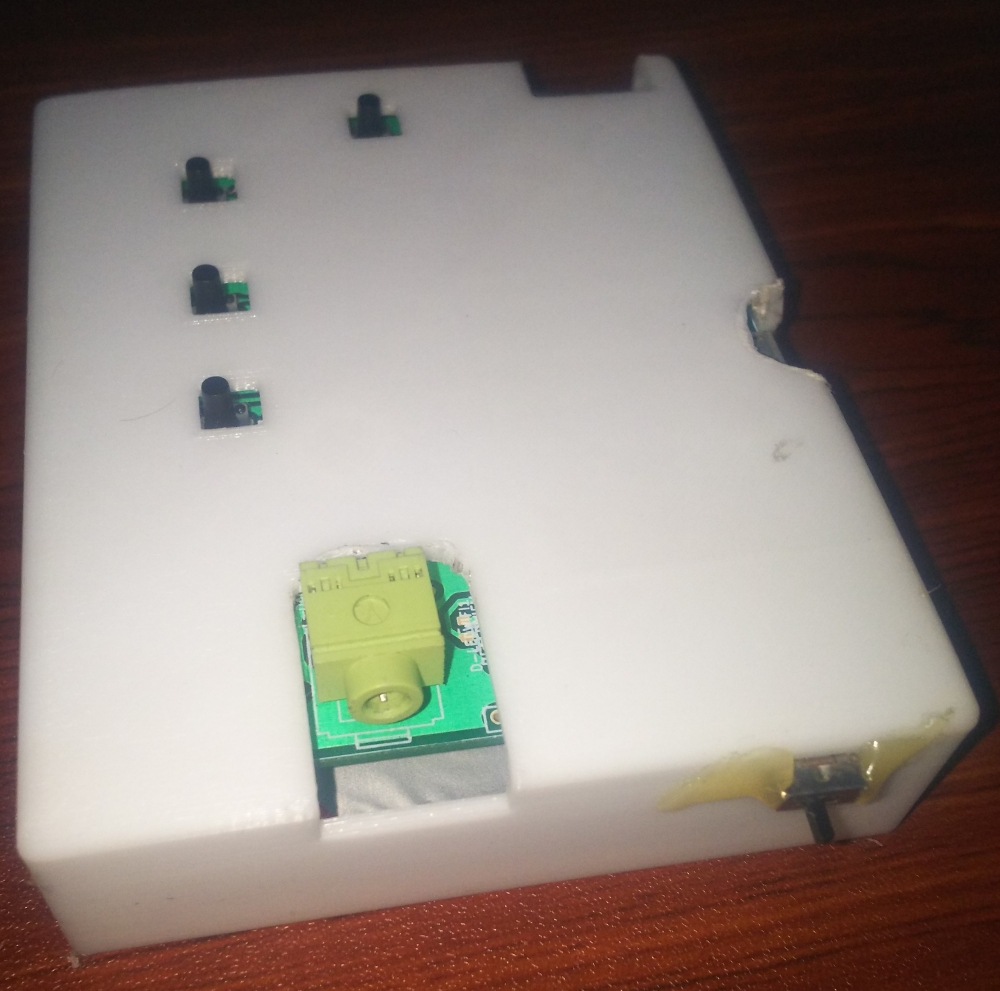
\includegraphics[width=150pt]{images/foto/unit}
			\caption{Unit Prototype}
		\end{figure}
	
		\item Kabel Micro-USB ke USB-A.
		\begin{figure}[!ht]
			\centering
			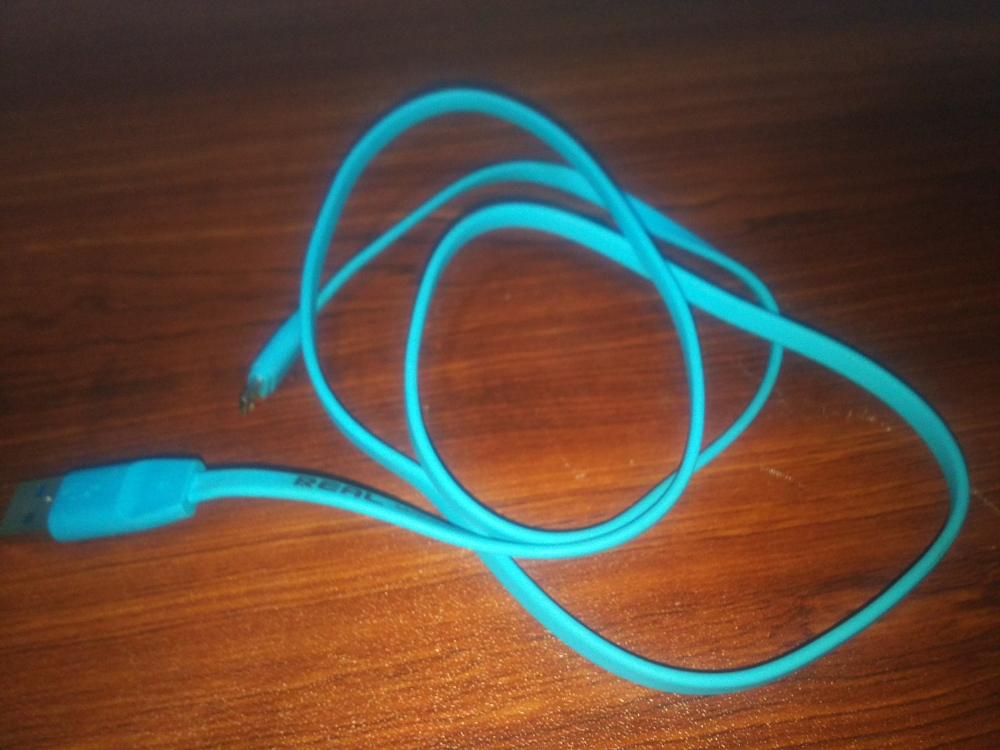
\includegraphics[width=150pt]{images/foto/kabel}
			\caption{Kabel USB}
		\end{figure}
	
		\item Wired-Headphone dengan impedansi tiap channel antara $32\Omega$ hingga $300\Omega$
		\begin{figure}[!ht]
			\centering
			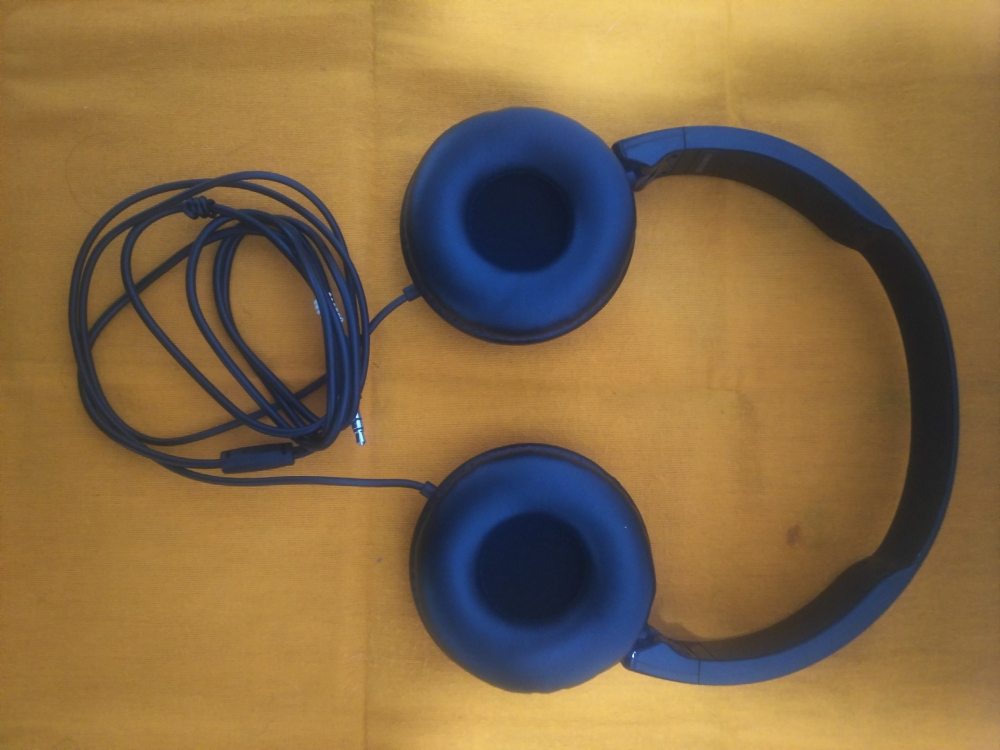
\includegraphics[width=150pt]{images/foto/phone}
			\caption{Kabel USB}
		\end{figure}
	
		\newpage
		\item Setup Uji KEMAR dan telah terkalibrasi.\\
		\textbf{Catatan}: Diasumsikan bahwa operator telah cukup familiar dalam detil teknis persiapan 
		maupun penggunaan unit uji KEMAR.
		\begin{figure}[!ht]
			\centering
			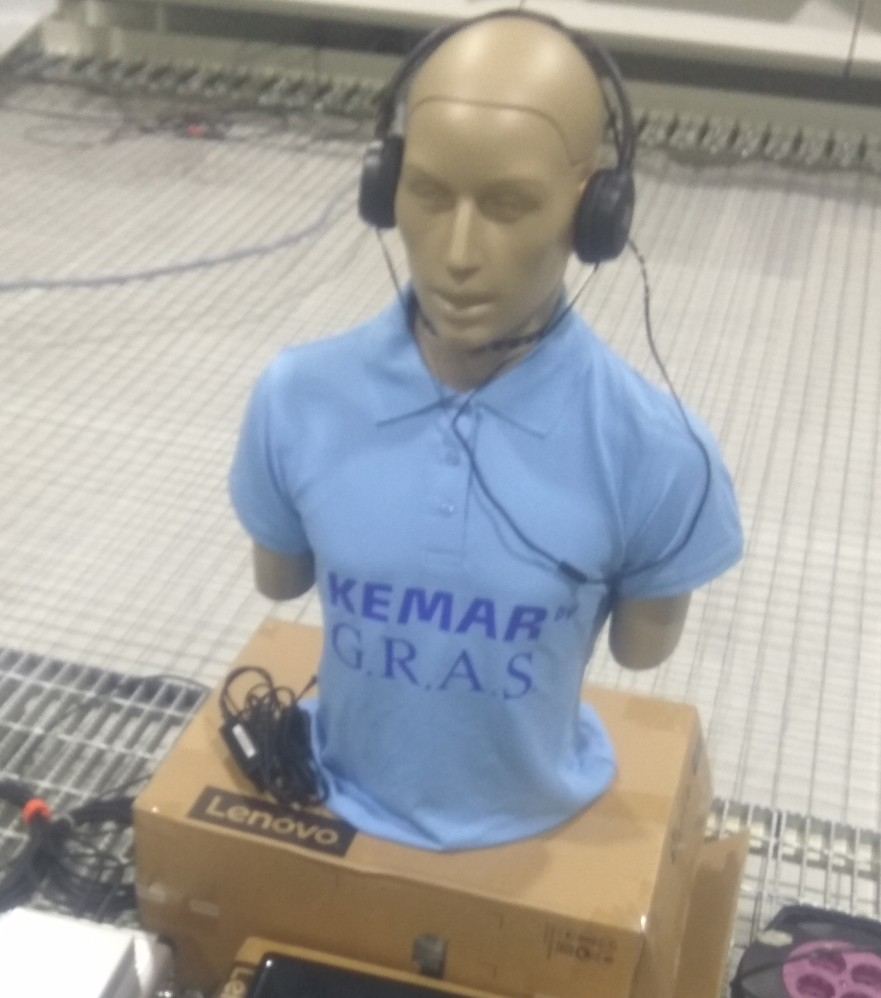
\includegraphics[width=150pt]{images/foto/kemar}
			\caption{Setup Kemar}
		\end{figure}
		
	\end{enumerate}

	\subsubsection{Software: Windows}
	
	Berikut adalah perangkat lunak yang perlu disiapkan untuk pengujian ini
	(panduan ini menggunakan Windows-7 32-bit sebagai contoh):
	
	\begin{enumerate}
		\item Install driver ARM USB-CDC.\\
		Untuk dapat menghubungkan unit prototype dengan komputer,
		diperlukan driver ARM USB-CDC untuk komunikasi serial.
		
		\begin{itemize}
			\item File installer (sesuaikan dengan bit OS).
			Dapat didownload di \url{http://intip.in/stm32tools}
			\begin{figure}[!ht]
				\centering
				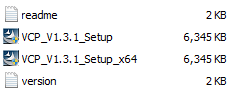
\includegraphics[width=200pt]{images/terminal/driver}
				\caption{Installer Driver}
			\end{figure}
		
			\item Instalasi driver (tanpa unit prototype terhubung) cukup mudah sebagaimana umumnya.
			\begin{figure}[!ht]
				\centering
				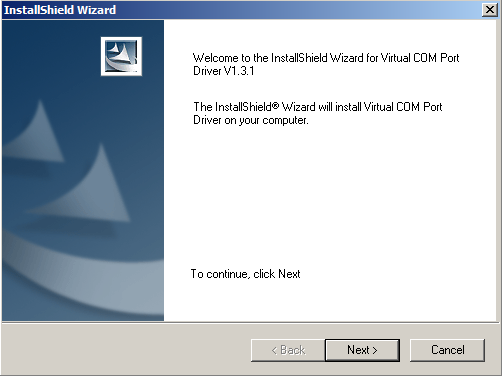
\includegraphics[width=200pt]{images/terminal/install_driver}
				\caption{Mulai instal driver}
			\end{figure}
		\end{itemize}
		
		\newpage
		\item Nyalakan dan hubungkan unit ke komputer.\\
		
		Berikut langkah-langkahnya:
		\begin{itemize}
			\item Hidupkan dengan switch pada sisi samping casing.
			\begin{figure}[!ht]
				\centering
				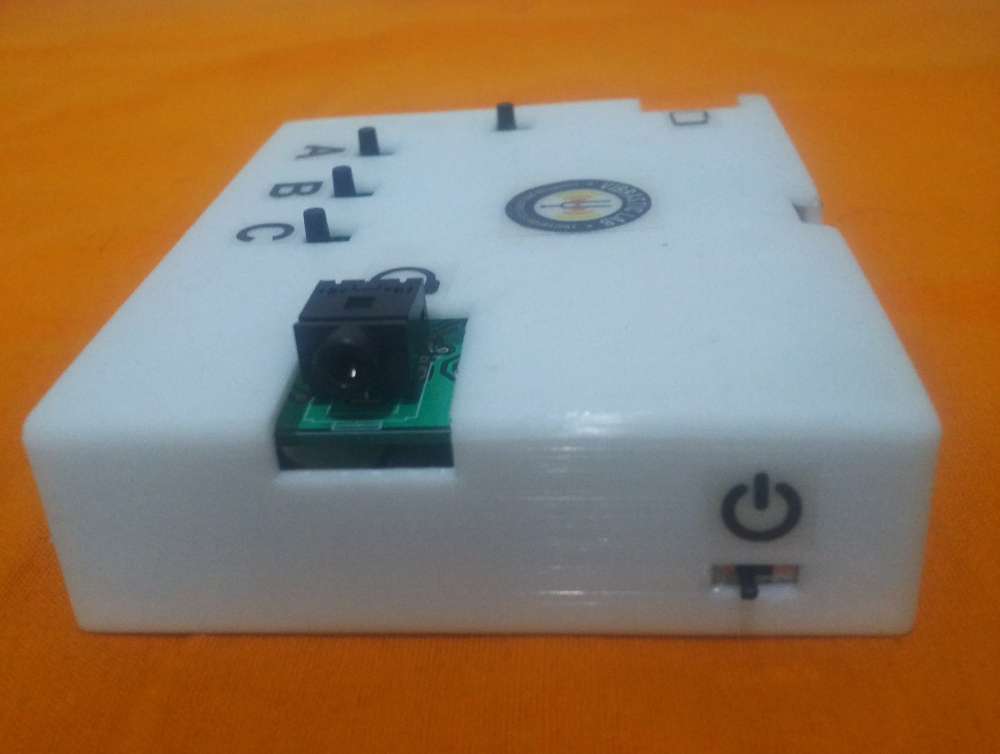
\includegraphics[width=150pt]{images/foto/pwrsw}
				\caption{Power Switch}
			\end{figure}
		
			\item Tunggu hingga LED biru, hijau, dan merah menyala
			bergantian sebagai tanda unit sudah standby
			
			\begin{figure}[!ht]
				\centering
				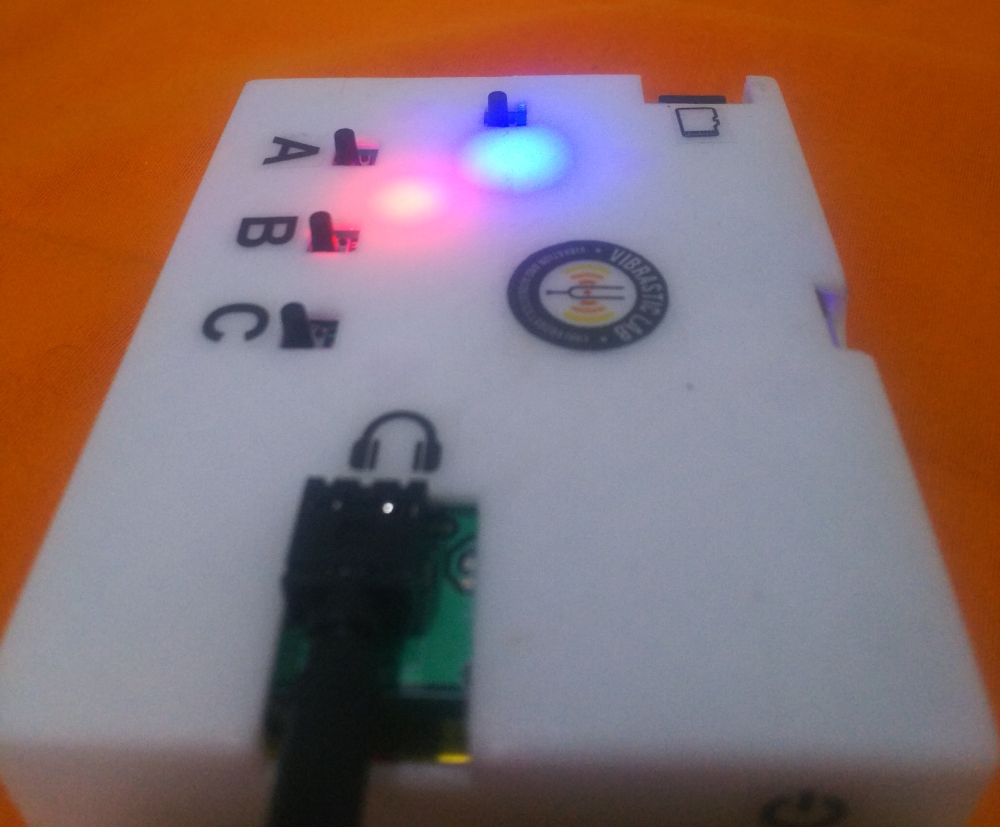
\includegraphics[width=150pt]{images/foto/standby}
				\caption{Unit Standby}
			\end{figure}
		
			\item Sambungkan unit prototype dengan komputer via kabel USB.
			
			\begin{figure}[!ht]
				\centering
				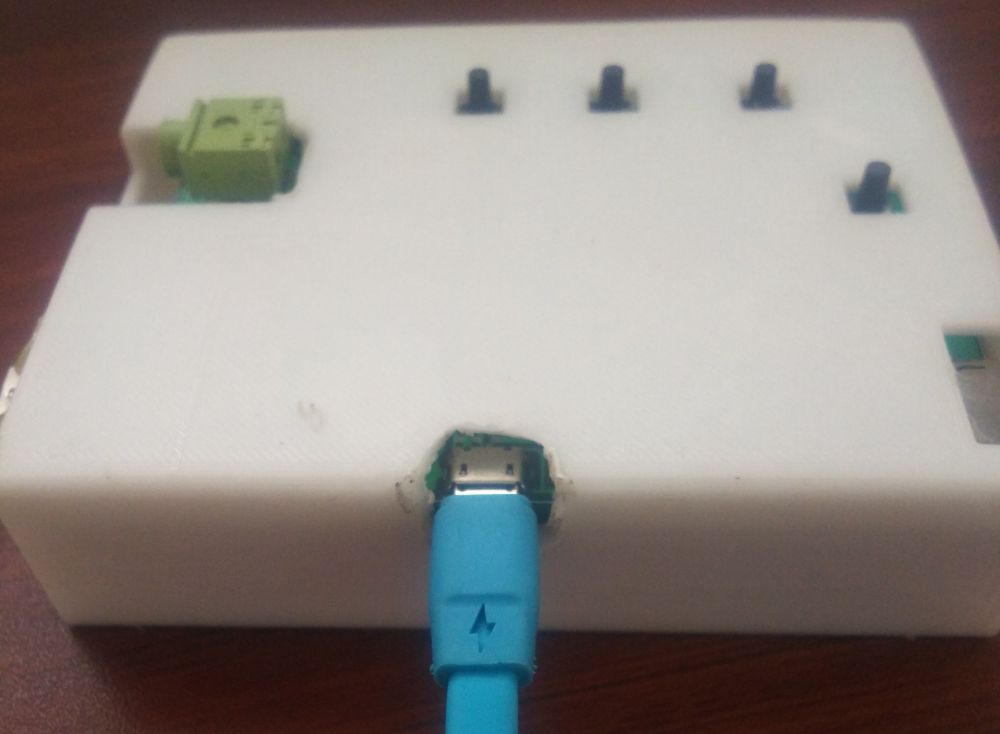
\includegraphics[width=150pt]{images/foto/konek}
				\caption{Konek Kabel USB}
			\end{figure}
			
		\end{itemize}
	
		\newpage
		\item Tunggu hingga driver selesai mengkonfigurasi otomatis
		
		\item Cek \textit{Device Manager} untuk mengetahui Nomor Serial-Port
		\begin{itemize}
			\item Buka run-command dialog dengan kombinasi keyboard (\keys{\WinKey + r})
			
			\item masukkan perintah \textbf{devmgmt.msc}.
			\begin{figure}[!ht]
				\centering
				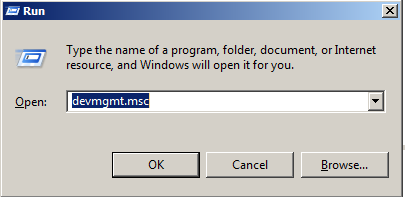
\includegraphics[width=200pt]{images/terminal/devicemgr}
				\caption{Memanggil Device Manager}
			\end{figure}
			
			\item Tekan (\keys{\return}) atau klik OK
			
			\item Cari entry \textit{Ports (COM and LPT)}.
			Catat nomor port untuk entry \textit{STMicroelectronics Virtual COM Port}.
			Dalam contoh ini, terkonfigurasi pada COM3.
			
			\begin{figure}[!ht]
				\centering
				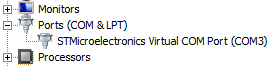
\includegraphics[width=200pt]{images/terminal/comport}
				\caption{Serial Komunikasi pada COM3}
			\end{figure}
		\end{itemize}
	
		\item Install Serial Terminal.
		Untuk dapat berkomunikasi via serial port, perlu diinstall serial terminal.
		Disini dicontohkan menggunakan \textit{Hercules}.
		
		\begin{itemize}
			\item Program terminal Hercules. Dapat didownload di \url{http://intip.in/stm32tools}
			\begin{figure}[!ht]
				\centering
				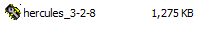
\includegraphics[width=200pt]{images/terminal/hercules}
				\caption{Hercules Terminal}
			\end{figure}
		
			\item Jalankan program Hercules.
			Jika muncul konfirmasi lisensi, cukup \textit{Close} saja.
			
			\item Pilih tab \textit{Serial}.
			\begin{figure}[!ht]
				\centering
				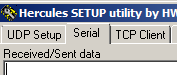
\includegraphics[width=200pt]{images/terminal/hercules_serial}
				\caption{Serial Terminal}
			\end{figure}
			
		\end{itemize}
	
		\newpage
		\item Test Komunikasi Serial
		\begin{itemize}
			\item Hercules Serial Terminal
			\begin{figure}[!ht]
				\centering
				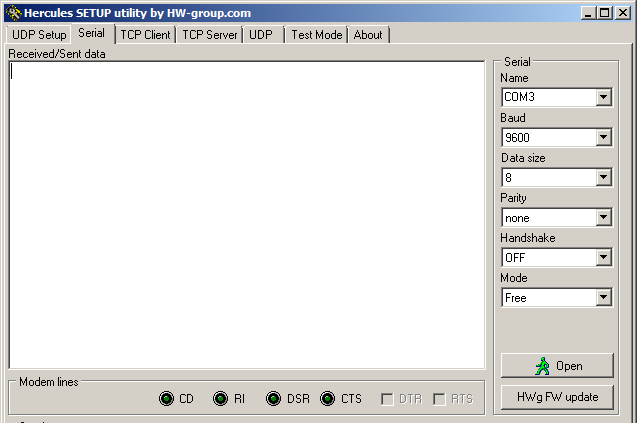
\includegraphics[width=250pt]{images/terminal/hercules_terminal}
				\caption{Hercules Serial Terminal}
			\end{figure}
		
			\item Setting Port pada Serial Terminal sebagai berikut
			\begin{itemize}
				\item Name     : COM3
				\item Baud     : 9600
				\item Data size: 8
				\item Parity   : none
			\end{itemize}
		
			\begin{figure}[!ht]
				\centering
				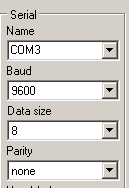
\includegraphics[width=100pt]{images/terminal/hercules_port}
				\caption{Pengaturan serial port}
			\end{figure}
		
			\item Klik Open (pastikan unit prototype sudah standby dan terhubung
			serta nama COM port sudah sesuai)
			
			\begin{figure}[!ht]
				\centering
				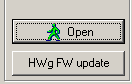
\includegraphics[width=100pt]{images/terminal/hercules_open}
				\caption{Open Serial Port}
			\end{figure}
			
			\item Kolom terminal akan menampilkan pesan:
			\begin{minted}[frame=lines,framesep=2mm,fontsize=\small]{bash}
Serial port COM3 opened
			\end{minted}
			
			\newpage
			\item Selanjutnya, pada kolom terminal,
			masukkan perintah berikut dan diakhiri dengan (\keys{\return})
			\begin{minted}[frame=lines,framesep=2mm,fontsize=\small]{bash}
info
			\end{minted}
			Serial akan menampilkan informasi kernel dan platform
			\begin{figure}[!ht]
				\centering
				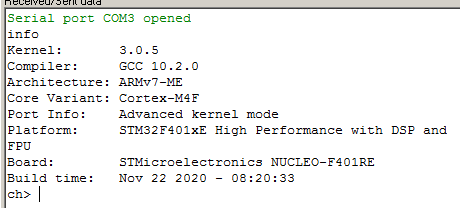
\includegraphics[width=300pt]{images/terminal/hercules_text}
				\caption{Informasi Platform}
			\end{figure}
		\end{itemize}
	\end{enumerate}

	\subsubsection{Software: Linux}
	
	Berikut adalah perangkat lunak yang perlu disiapkan untuk pengujian ini
	(panduan ini menggunakan Ubuntu sebagai contoh alternatif):
	
	\begin{enumerate}
		\item Instalasi Driver.\\
		Untuk driver sudah terintegrasi dengan kernel Linux 5.0 ke atas.
		Untuk mengetahui versi kernel dapat menggunakan perintah pada terminal Ubuntu:
		\begin{minted}[frame=lines,framesep=2mm,fontsize=\small]{bash}
uname -a
		\end{minted}
		
		\item Nyalakan dan hubungkan unit ke komputer.\\
		Prosedurnya sama dengan panduan untuk Windows.
		
		\item Serial Port
		\begin{itemize}
			\item Untuk mengecek USB telah terdaftar atau belum,
			dapat digunakan perintah berikut pada terminal Ubuntu:
			\begin{minted}[frame=lines,framesep=2mm,fontsize=\small]{bash}
lsusb
			\end{minted}
			Hasilnya akan menampilkan daftar USB yang terpasang.
			Pastikan ada \textit{STMicroelectronics Virtual COM Port}.
			\begin{figure}[!ht]
				\centering
				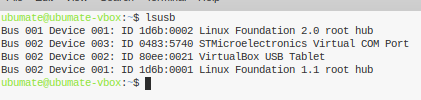
\includegraphics[width=300pt]{images/terminal/ubu_usbport}
				\caption{Daftar USB terpasang}
			\end{figure}
			
			\newpage
			\item Untuk mendapatkan nomor serial port
			dapat digunakan perintah berikut pada terminal Ubuntu:
			\begin{minted}[frame=lines,framesep=2mm,fontsize=\small]{bash}
ls /dev/ttyACM*
			\end{minted}
			Hasilnya akan menampilkan port USB standar ACM-CDC.
			\begin{figure}[!ht]
				\centering
				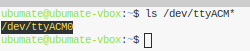
\includegraphics[width=300pt]{images/terminal/ubu_acmport}
				\caption{nomor Serial Port}
			\end{figure}
		\end{itemize}
		
		
	\end{enumerate}
	
	
\end{document}
